\section{Simulation Analysis}
\label{sec:simulation}

By creating a \textit{Ngspice} script, we started out by trying different configurations for the envelope detector. We ended up choosing to move on with a full-wave bridge rectifier.
Then, we joined the envelope detector with a voltage regulator until we had satisfactory results. All of this looking at 10 periods after the initial transient period, and using the default diode model.
Finally, we added \textit{Ngspice} commands to calculate the main quality outputs: the average and the ripple. The results will be shown later, side-by-side with the theoretical analysis' results.


% \begin{figure*}[h]
%     \centering
%     \begin{subfigure}{0.23\textwidth}
%         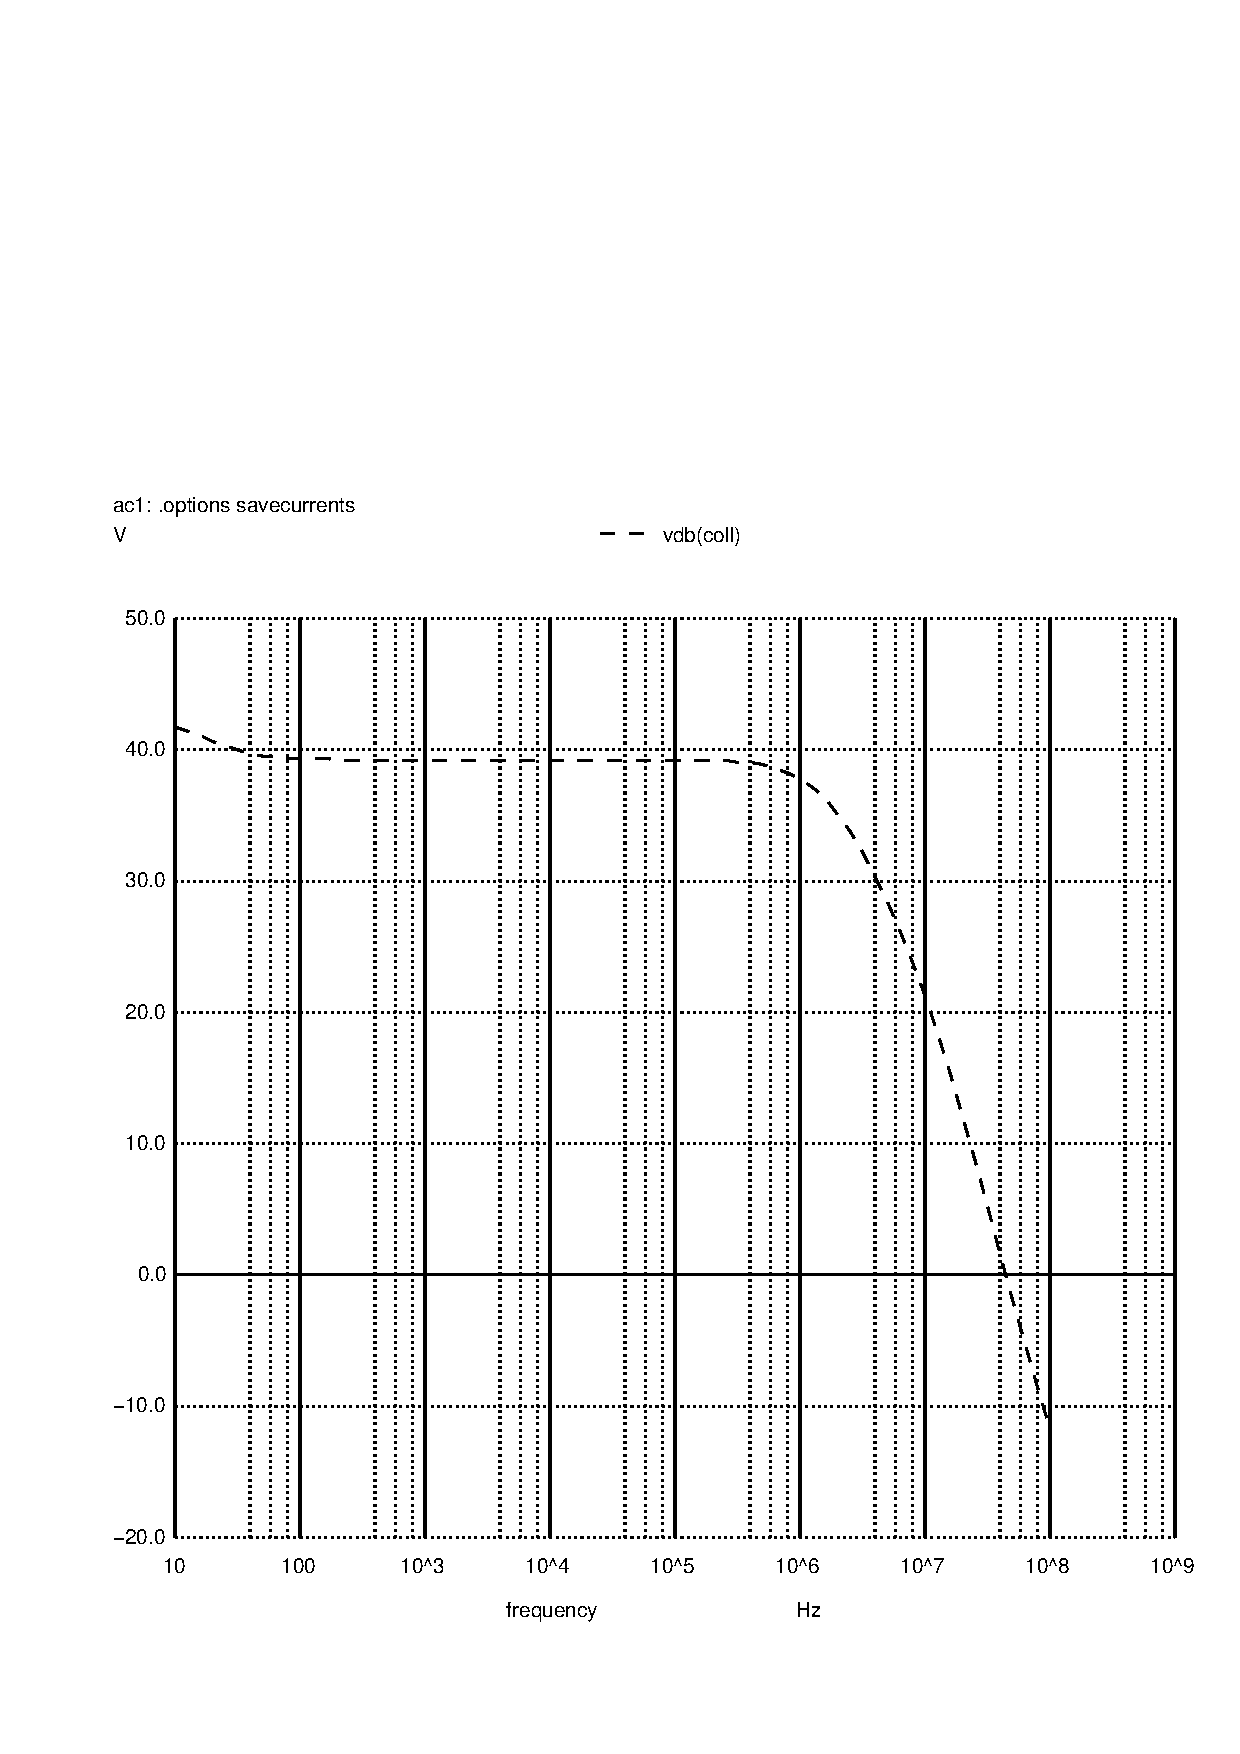
\includegraphics[width=\linewidth, clip]{vo2f.pdf}
%         \label{fig:output1}
%     \end{subfigure}
%     \begin{subfigure}{0.23\textwidth}
%         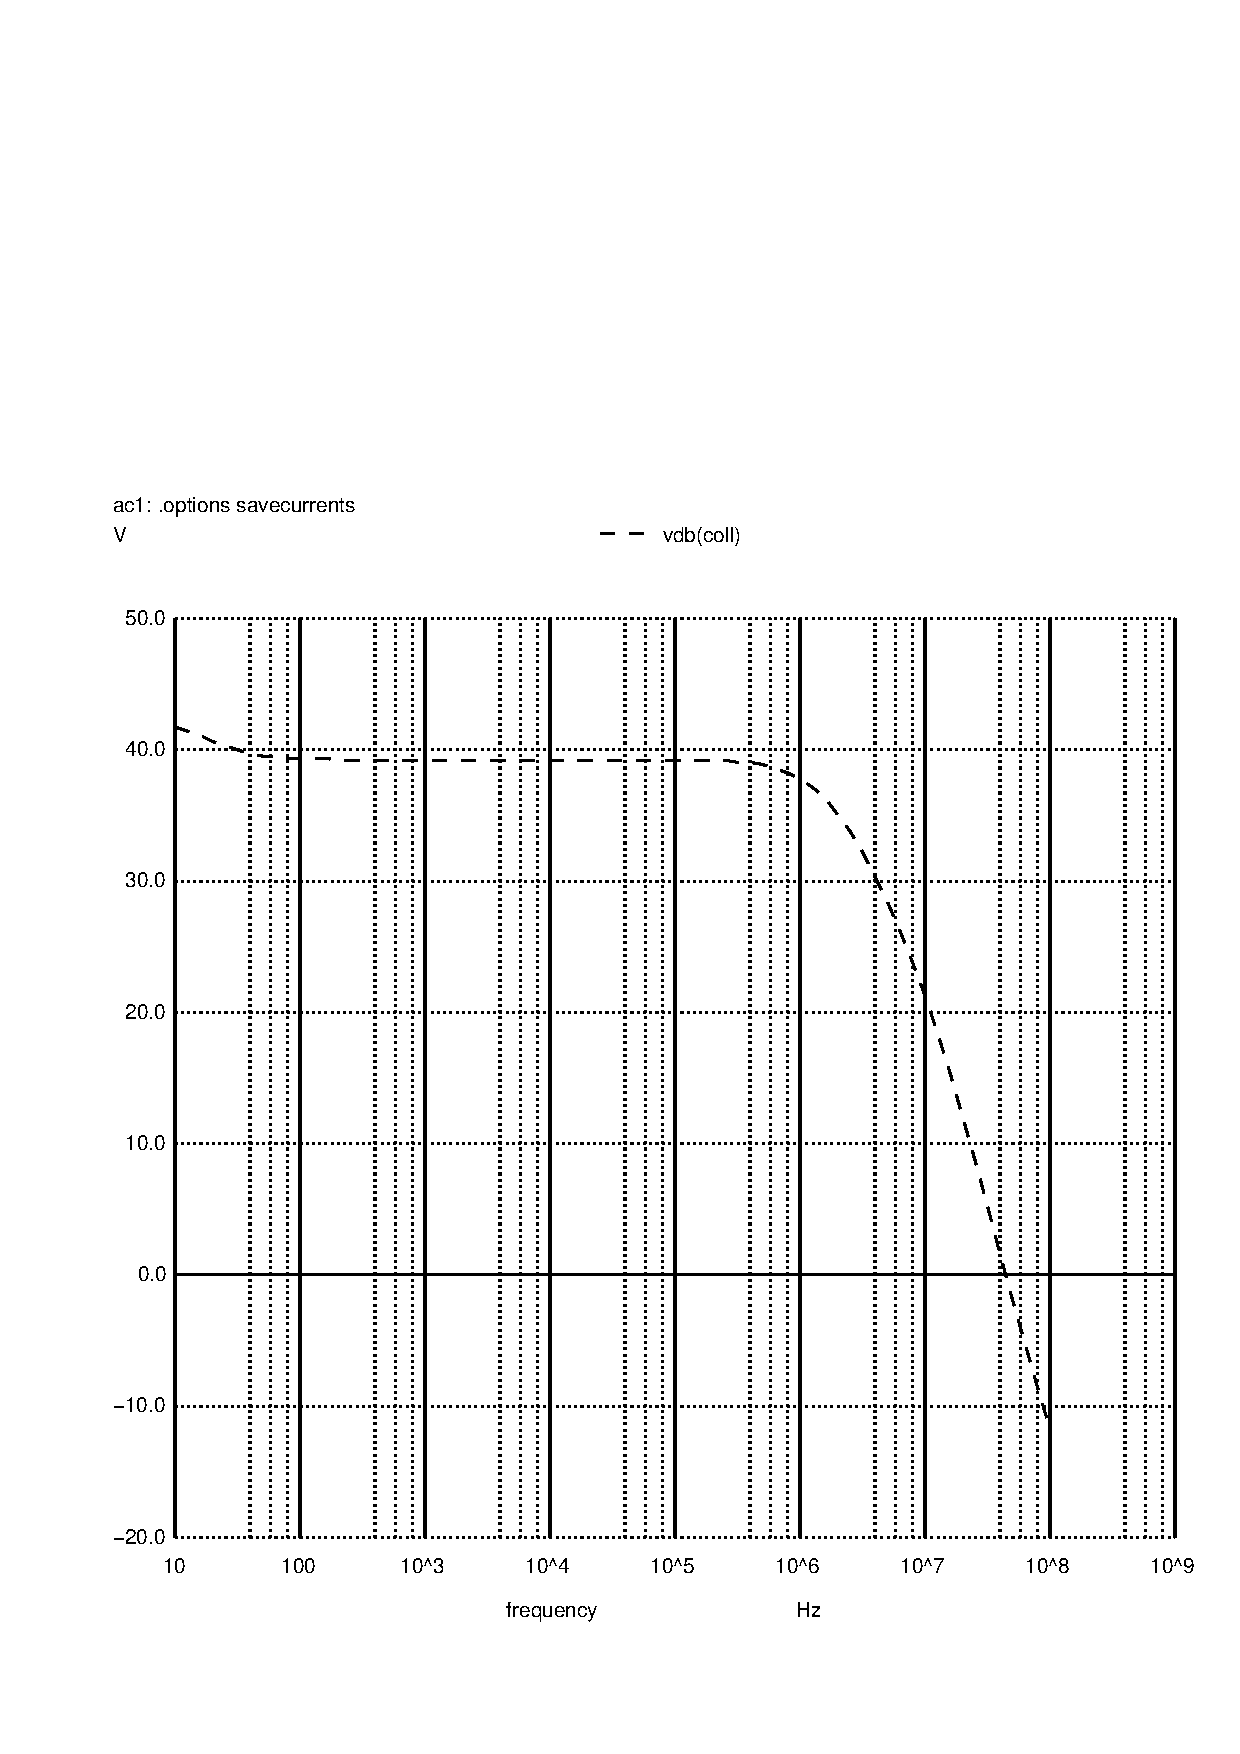
\includegraphics[width=\linewidth, clip]{vo1f.pdf}
%         \label{fig:output2}
%     \end{subfigure}
%     \caption{\small $V_Out - 12$ - measure of the output DC deviation + AC component (left - simulation; right - theoretical )}
%     \label{output_deviation}
% \end{figure*}

\begin{figure}
    \centering
    \begin{subfigure}{.5\textwidth}
        \centering
        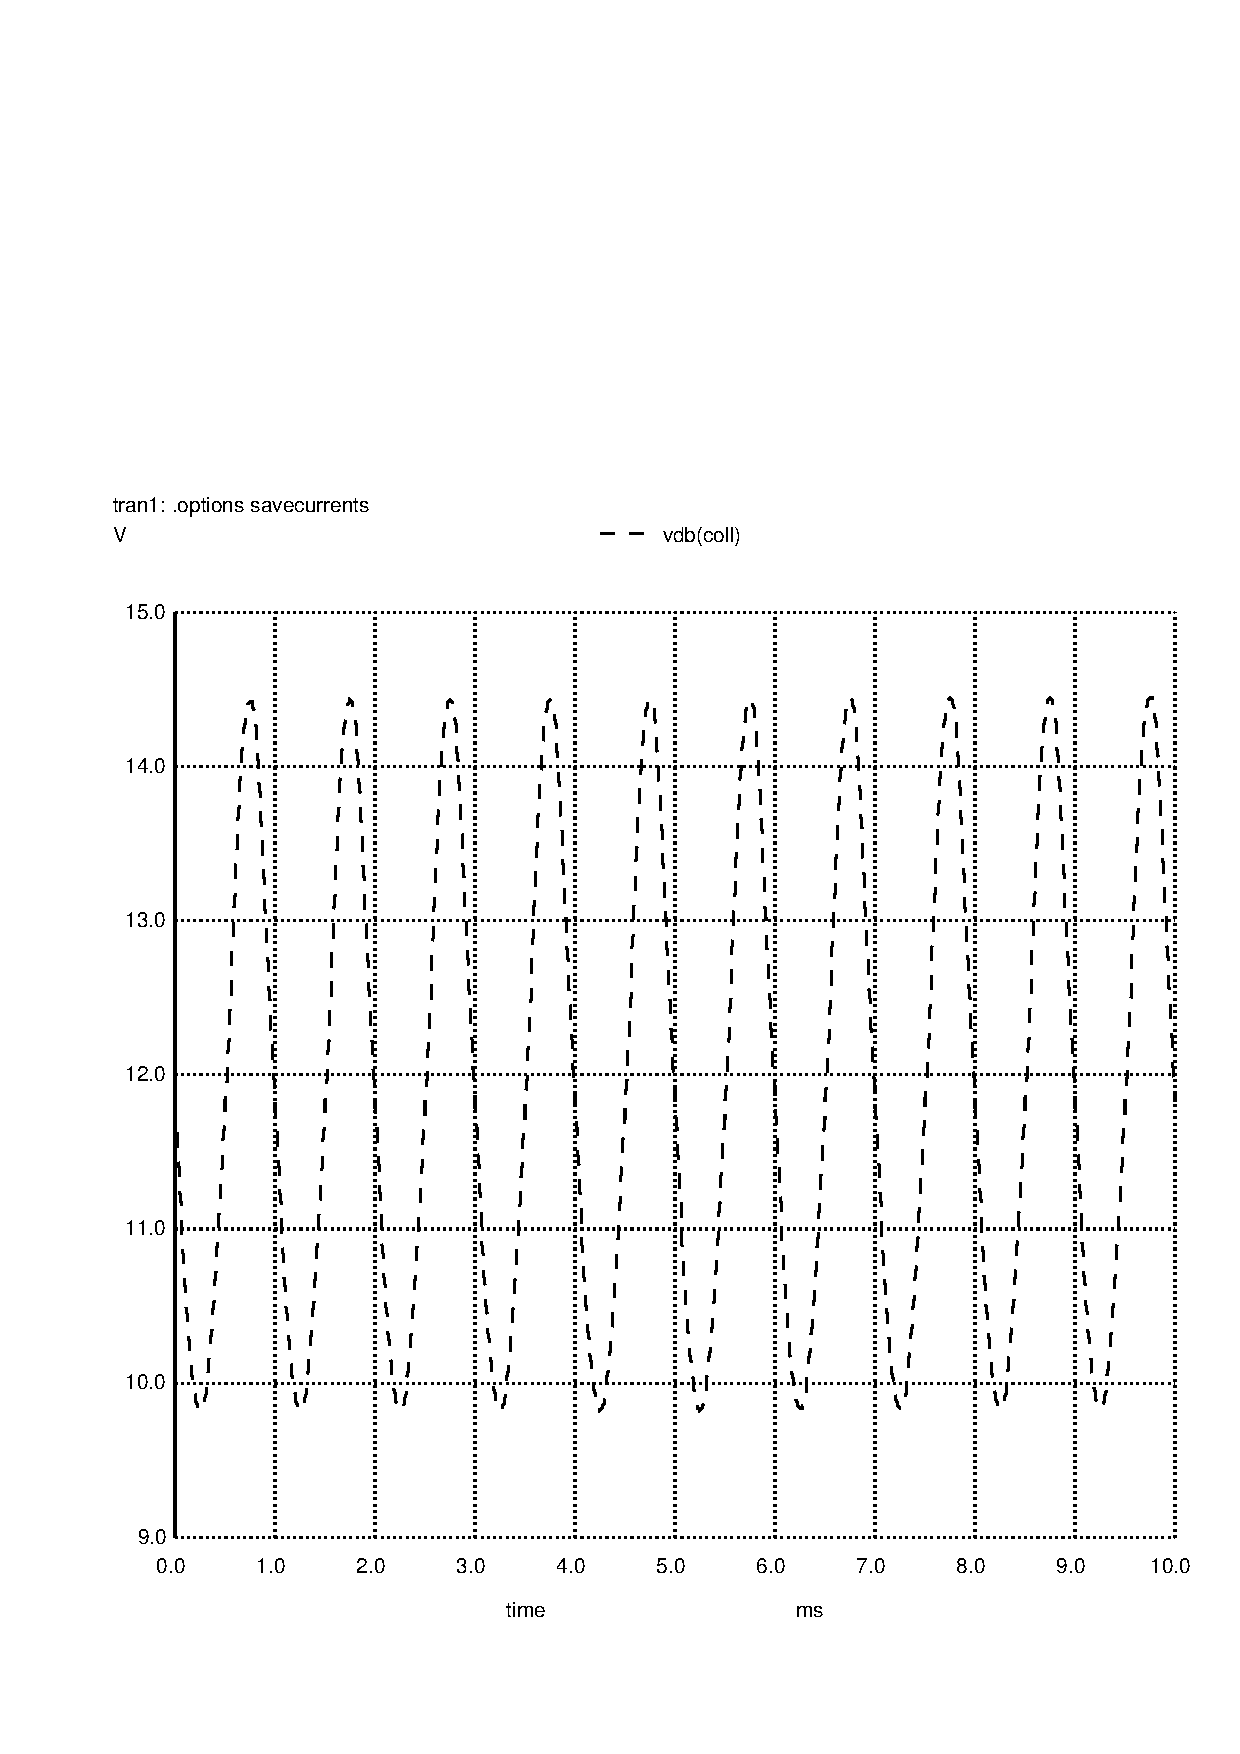
\includegraphics[width=.4\linewidth]{vo1.pdf}
        \caption{A subfigure}
        \label{fig:sub1}
    \end{subfigure}%
    \begin{subfigure}{.5\textwidth}
        \centering
        \includegraphics[width=.4\linewidth]{gainACtotal.eps}
        \caption{A subfigure}
        \label{fig:sub2}
    \end{subfigure}
    \caption{A figure with two subfigures}
    \label{fig:test}
\end{figure}


\begin{table}
    \parbox{.45\linewidth}{
        \centering
        \begin{tabular}{|c|c|}
            \hline
            {\bf Name} & {\bf Value [A or V]} \\ \hline
            gm1 & 3.577156e-01\\ \hline
$r pi 1$ & 4.995588e+02\\ \hline
r01 & 7.793900e+03\\ \hline
AV1 & -2.627909e+02\\ \hline
$AV1_{DB}$ & 4.839221e+01\\ \hline
ZI1& 4.844336e+02\\ \hline
ZO1 & 8.862848e+02\\ \hline

        \end{tabular}
        \label{tab:GainStage_AC}
        \caption{Results of Nodal Analysis of the circuit for t < 0. A variable that begins  with \textit{I} names a \textit{current} in \textit{Ampere}; the ones that start with \textit{V} name a \textit{voltage} in \textit{Volt}}
    }
    \hfill
    \parbox{.45\linewidth}{
        \centering
        \begin{tabular}{|c|c|}
            {\bf Name} & {\bf Value [A or V]} \\ \hline
            VEQ & 2.400000e+00\\ \hline
IB1 & 5.004416e-05\\ \hline
IC1 & 8.942891e-03\\ \hline
VEQ & 8.992935e-03\\ \hline
VE1 & 8.992935e-01\\ \hline
V01 & 3.057109e+00\\ \hline
VCE & 2.157816e+00\\ \hline

            \hline
        \end{tabular}
        \label{tab:GainStage_OP}
        \caption{Table with results from Ngspice to find out the voltages and currents in each node and branch. A variable that begins  with \textit{I} names a \textit{current} in \textit{Ampere}; the ones that start with \textit{V} name a \textit{voltage} in \textit{Volt} }
    }
\end{table}



